\documentclass{ctpro}
\usepackage{tikz}

\title{ACM 算法与微应用实验室 2022 年 4 月月赛题目}
\date{2022 年 5 月 1 日}

\begin{document}

\maketitle
\addproblem{FMVP}{1000}{256}{传统}{AgOH}
\addproblem{最强阵容}{1000}{256}{传统}{AgOH}
\addproblem{八保舟}{1000}{256}{传统}{AgOH}
\addproblem{自古红蓝}{1000}{256}{传统}{AgOH}
\addproblem{5Yqg5a+G6YCa5L+h}{1000}{256}{传统}{AgOH}
\addproblem{K-prime seive 2}{1000}{256}{传统}{Tifa}

\section*{比赛信息}

\ctinfotab{ACM 个人赛}{C/C++,~Python,~Java}{3}

\section*{题目概况}

\problemtab

\section*{编译命令}

参见 OJ 帮助

\section*{注意事项}

\begin{itemize}
    \item C/C++ 中函数 \verb|main()| 的返回值类型必须是 \verb|int|,程序正常结束时的返回值必须是 $0$。
    \item C/C++ 代码必须完全符合 GNU C/C++ 标准,不能使用诸如绘图、Win32API、中断调用、硬件操作或与操作系统相关的API。
    \item C/C++ 代码中允许使用 STL 类库。
\end{itemize}

\paragraph*{} 祝大家取得好成绩!

\makeproblem
\section*{题目描述}

在 4 月 26 日刚刚结束的 CBA 总决赛中,辽宁本钢队以 4:0 的大比分击败了浙江广厦队,获得了队史第二座总冠军奖杯。

根据 CBA 联赛的规则,总决赛系列赛中场均 SPR 值最高的球员将会获得总决赛 MVP 的称号。现给出每名球员每场比赛的 SPR 值,请你帮 CBA 联盟评选出谁是总决赛 MVP。

\section*{输入格式}

第一行,一个整数 $n~(1 \leq n \leq {10}^5)$,代表共有 $n$ 名球员有资格评选总决赛 MVP。

接下来 $n$ 行,每行一个字符串和四个实数,依次代表球员的名字和其总决赛每场比赛的 SPR 值。

数据保证:

\begin{itemize}
    \item 球员名字长度不超过 $20$,只由大小写字母构成,且内部不存在空格;
    \item SPR 值的绝对值不超过 $20$;
    \item 不会出现两个场均 SPR 值相同的球员。
\end{itemize}

\section*{输出格式}

一行,一个字符串,格式为:\texttt{x is the FMVP!},\texttt{x} 为总决赛 MVP 球员的名字。

\section*{输入输出样例}

\testcasetab
{
    10\par
    FuHao 10.5 5.8 -1.7 6.1\par
    ZhaoJiwei 4.8 7.4 5.4 18.9\par
    ZhouJuncheng 3.8 2.5 0 -2.3\par
    ZhangZhenlin 3.1 5.6 5.7 3.5\par
    CongMingchen 1.8 1.3 -2.4 0\par
    GuoAilun 6.9 -8.3 7.6 0.1\par
    KyleFogg 2.2 15.5 -0.1 3.8\par
    LiXiaoxu 2.4 -0.8 1.1 4.5\par
    EricMoreland 5.7 10.3 6.8 5.5\par
    HanDejun 0 3.3 6.4 4.4
}
{
    ZhaoJiwei is the FMVP!
}

\clearpage
\section*{说明/提示}

【样例解释】

球员 ZhaoJiwei 的场均 SPR 值为:$\cfrac{4.8+7.4+5.4+18.9}{4} = 9.125$,为场均 SPR 最高的球员,故球员 ZhaoJiwei 为总决赛 MVP。

\makeproblem
\section*{题目描述}

国际篮球联合会(FIBA)于 2020 年发布的规则的第 1.1 条部分内容如下:

\begin{quote}
    \textbf{1.1 Basketball game}

    Basketball is played by 2 teams of 5 players each.
\end{quote}

即篮球比赛是由两队各派出五人进行对垒。

每名球员有两个能力值:进攻效率和防守效率。一个五人阵容的实力为 $\cfrac{\text{五人进攻效率之和}}{\text{五人防守效率之和}}$。

给定辽宁本钢队所有球员的进攻效率和防守效率,现在需要在所有球员中选出五个人组成一个五人阵容,请问这个阵容的实力的最大值是多少?

\section*{输入格式}

第一行,一个整数 $n~(5 \leq n \leq {10}^5)$,代表辽宁本钢队共有多少名球员。

接下来 $n$ 行,每行两个整数 $a_i,b_i~(1 \leq a_i,b_i \leq {10}^7)$,分别代表一名球员的进攻效率和防守效率。

\section*{输出格式}

一行,一个实数,代表能选出的实力最大的阵容的实力,保留 $6$ 位小数。

\section*{输入输出样例}

\testcasetab
{
    6\par
    8 9\par
    2 9\par
    10 3\par
    1 7\par
    4 8\par
    10 5
}
{
    1.031250
}

\testcasetab
{
    10\par
    20 19\par
    9 19\par
    1 9\par
    1 8\par
    11 6\par
    8 14\par
    9 14\par
    8 20\par
    15 2\par
    10 2
}
{
    1.540541
}

\section*{说明/提示}

【样例解释 \#1】

最优选法为选择第 $1$、$2$、$5$、$6$、$7$ 名球员。

【样例解释 \#2】

最优选法为选择第 $1$、$3$、$4$、$5$、$6$ 名球员。

\makeproblem
\section*{题目描述}

史尔特尔非常喜欢吃冰淇淋,夏天到了,她缠着博士给她买了好多好多个冰淇淋。

每个冰淇淋都有一个快乐值 $h_i$,如果史尔特尔吃掉了这个冰淇淋,那么她自己的快乐值就会加上这个冰淇淋的快乐值。

史尔特尔只能一个一个地吃冰淇淋,但是夏天很热,冰淇淋会很快地融化,史尔特尔每吃掉一个冰淇淋,其他冰淇淋就会因为融化导致其快乐值 $-1$,每个冰淇淋的快乐值最小只会扣减到 $0$。

博士想让史尔特尔变得非常高兴,这样才能让她接受被医疗干员簇拥着永续黄昏的任务。史尔特尔初始的快乐值为 $42$,博士会给你 $q$ 次询问,每次询问一个区间 $[l,r]$,你需要帮博士算出只给史尔特尔吃第 $l,l+1,\cdots,r$ 个冰淇淋后史尔特尔能达到的最大快乐值是多少。

\section*{输入格式}

第一行,一个整数 $n,q~(1 \leq n,q \leq {10}^4)$,分别代表共有 $n$ 个冰淇淋以及博士的询问个数。

第二行,$n$ 个整数 $h_i~(1 \leq h_i \leq {10}^5)$,代表每个冰淇淋的快乐值。

接下来 $q$ 行,每行两个整数 $l,r~(1 \leq l \leq r \leq n)$,代表博士的一次询问。

\section*{输出格式}

共 $q$ 行,第 $i$ 行为博士的第 $i$ 次询问的答案。

\section*{输入输出样例}

\testcasetab
{
    5 5\par
    1 3 5 7 9\par
    1 3\par
    2 4\par
    3 5\par
    1 4\par
    2 5
}
{
    49\par
    54\par
    60\par
    54\par
    60\par
}

\makeproblem
\section*{题目描述}

给定一个 $1 \times n$ 的矩形格条,你需要对每个格子涂上红色或者蓝色。但是两个红色的格子不允许相邻,请问共有多少种涂色的方案?

因为答案可能很大,你只需要输出答案对 $998244353$ 取模的结果即可。

\section*{输入格式}

一行,一个整数 $n~(1 \leq n \leq {10}^{18})$。

\section*{输出格式}

一行,一个整数,代表答案。

\section*{输入输出样例}

\testcasetab
{
    3
}
{
    5
}

\testcasetab
{
    2333333
}
{
    394054407
}

\section*{说明/提示}

【样例解释 \#1】

$5$ 种合法的涂色方法分别为:红蓝红,红蓝蓝,蓝红蓝,蓝蓝红,蓝蓝蓝。

\makeproblem
\section*{题目描述}

有 $n$ 台计算机,编号从 $1$ 到 $n$,这 $n$ 台计算机之间有若干条加密的连接,每条连接都是双向的,且任意两台计算机之间都可以通过若干台计算机间接相连。若计算机 $i$ 和计算机 $j$ 有一条连接使得二者直接相连,则这条连接有权值 $w_{ij}$。计算机 $i$ 向其他计算机请求一次内容的过程如下:

\begin{itemize}
    \item 计算机 $i$ 生成数据包
    \item 设与计算机 $i$ 存在连接的计算机编号分别为 $i_1,i_2,...,i_s$,则计算机 $i$ 新建 $s$ 个线程,第 $x$ 号线程花费 $w_{i,i_x}$ 的时间加密数据包,加密完成后发送数据包。
    \item 计算机 $i_x$ 在收到数据包后,花费 $w_{i,i_x}$ 的时间解密数据包。
    \item 若请求的内容不在计算机 $i_x$ 上,则计算机 $i_x$ 向所有与其存在连接的计算机(不包括计算机 $i$ )请求相同的内容,在收到内容后,则按照请求的内容在计算机 $i_x$ 的情况继续进行。
    \item 若请求的内容在计算机 $i_x$ 上,则计算机 $i_x$ 生成包含请求内容的数据包,并花费 $w_{i,i_x}$ 的时间加密数据包,加密完成后向计算机 $i$ 发送数据包。
    \item 计算机 $i$ 收到计算机 $i_x$ 的数据包后仍需花费 $w_{i,i_x}$ 的时间解密数据包才能获得请求的内容。
\end{itemize}

因为通信过程中的耗时主要在加解密的过程,所以通信的时间只考虑加解密的时间。

Tifa 认为这个网络的通信时间过长,所以 Tifa 搭建了一个加速服务器,可以使得一对直接相连的计算机之间的通信变为与服务器进行未加密的通信,从而使这一对计算机之间的权值从 $w_{ij}$ 变为 $0$。由于 Tifa 技术水平的限制,这个服务器只能对 $k$ 条连接进行加速。

已知请求的内容在计算机 $n$ 上,Tifa 想知道从计算机 $1$ 请求一次内容的最短耗时是多少。

\section*{输入格式}

第一行,三个整数 $n,m,k,~(1 \leq n \leq {10}^4,~1 \leq m \leq 5 \times {10}^4,~1 \leq k \leq 10)$,分别代表图的结点数量,边数量和 $k$ 的值。

接下来 $m$ 行,每行两个整数 $u_i,v_i,w_i~(1 \leq u_i,v_i \leq n,~1 \leq w_i \leq {10}^3)$,代表 $u_i,v_i$ 两个结点之间存在一条边权为 $w_i$ 的边。

\section*{输出格式}

第一行,一个整数,代表答案。

如果答案为 $0$,则需在第二行输出 \verb|Identified as: Purely Network Connection.|,否则不要输出任何内容。

\section*{输入输出样例}

\testcasetab
{
    5 5 1\par
    1 2 2\par
    2 3 2\par
    1 4 3\par
    4 5 3\par
    3 5 2
}
{
    12
}

\testcasetab
{
    2 1 1\par
    1 2 3
}
{
    0\par
    \small Identified as: Purely Network Connection.
}

\section*{说明/提示}

【样例解释 \#1】

$5$ 台计算机之间的连接关系如下:

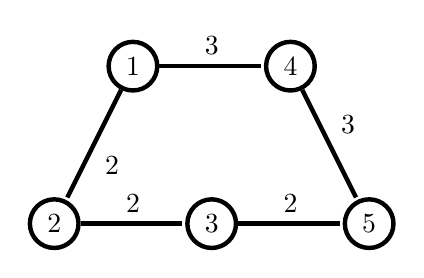
\begin{tikzpicture}[shorten >=1pt, auto, node distance=3cm, ultra thick,
    node_style/.style={circle,draw=black},
    edge_style/.style={draw=black, ultra thick}]
 
    \node[node_style] (v1) at (1,2) {1};
    \node[node_style] (v2) at (0,0) {2};
    \node[node_style] (v3) at (2,0) {3};
    \node[node_style] (v4) at (3,2) {4};
    \node[node_style] (v5) at (4,0) {5};
    \draw[edge_style] (v1) edge node{2} (v2);
    \draw[edge_style] (v2) edge node{2} (v3);
    \draw[edge_style] (v1) edge node{3} (v4);
    \draw[edge_style] (v4) edge node{3} (v5);
    \draw[edge_style] (v3) edge node{2} (v5);
\end{tikzpicture}

当 Tifa 使用加速服务器使 $(1,4)$ 或 $(4,5)$ 两台计算机之间的通信变为与服务器进行未加密的通信时,请求内容的最短耗时为 $12$,为所有加速方案中的最优解。

\makeproblem
\section*{题目描述}

给定定义如下:

\begin{definition}[$k$-素数]
    恰好能表示为 $k$ 个素数乘积的数称为 $k$-素数
\end{definition}

对于给定的区间 $[l,r]$,请问 $[l,r]$ 中有多少 $k$-素数?

\section*{输入格式}

多组数据。

第一行为一个整数 $t~(1 \leq t \leq 100)$,表示数据组数。

接下来 $t$ 行每行有三个整数 $l,r,k~(1 \leq l<r \leq {10}^{12},~r-l\leq {10}^6,~0 \leq k \leq r)$,含义同描述。

\section*{输出格式}

每组数据输出一行,每行输出一个数,为 $[l,r]$ 中所有 $k$-素数的个数。

\section*{输入输出样例}

\testcasetab
{
    4\par
    1 1 1\par
    1 20 1\par
    1 10 2\par
    1 30 3
}
{
    0\par
    8\par
    4\par
    7
}

\end{document}
